% Preamble
% ---
\documentclass{article}

% Packages
% ---
\usepackage{amsmath} % Advanced math typesetting
\usepackage[utf8]{inputenc} % Unicode support (Umlauts etc.)
\usepackage[ngerman]{babel} % Change hyphenation rules
\usepackage{hyperref} % Add a link to your document
\usepackage{graphicx} % Add pictures to your document
\usepackage{listings} % Source code formatting and highlighting
\usepackage{booktabs}

\renewcommand{\figurename}{Figure}
%\usepackage[labelsep=endash]{caption}

\usepackage{xcolor}
\lstset { %
    language=C++,
    backgroundcolor=\color{black!5}, % set backgroundcolor
    basicstyle=\footnotesize,% basic font setting
}



\title{%
	MA226 : Monte-Carlo Simulation\\
	 Generating Standard Normal Distritution\\
	 \large Assignment 6}

\date{09-03-2017}

\author{%
	Turkhade Hrushikesh Pramod\\
	150123044	}	

\begin{document}

	\maketitle
	\pagenumbering{gobble}
	
	\newpage
	\pagenumbering{arabic}
	
	\section{Problem 1}
	\paragraph{}
		We have to generate sample from standard normal distribution using Box-Muller Transform and Marsaglia-Bray Method.
				
	\subsection{Source code of the solution}
		\lstinputlisting[language=R,firstline=1]{code/que1.R}
	
	\subsection{Generated Histograms}
			\begin{figure}
  			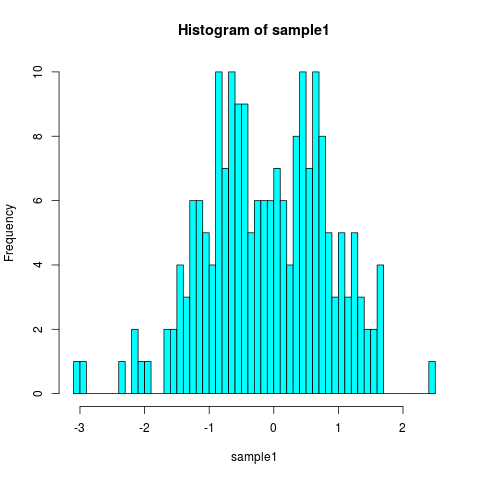
\includegraphics[width=\linewidth]{pic/que1_hund_1.png}
 			 \caption{Using Box-Muller for 100 sample} 
  			\label{fig:hist1}
		\end{figure}
	
			\begin{figure}
  			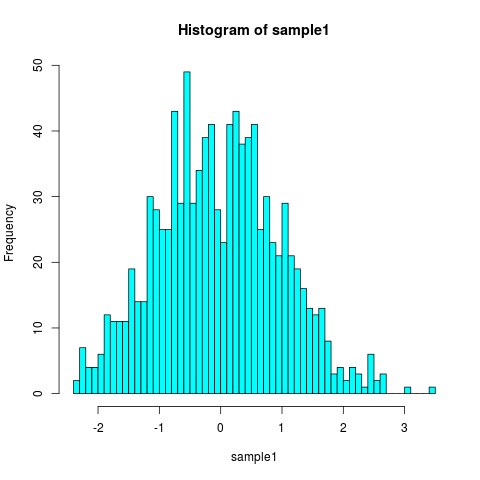
\includegraphics[width=\linewidth]{pic/que1_five-hund_1.png}
 			 \caption{Using Box-Muller for 500 sample} 
  			\label{fig:hist1}
		\end{figure}
	

			\begin{figure}[!ht]
  			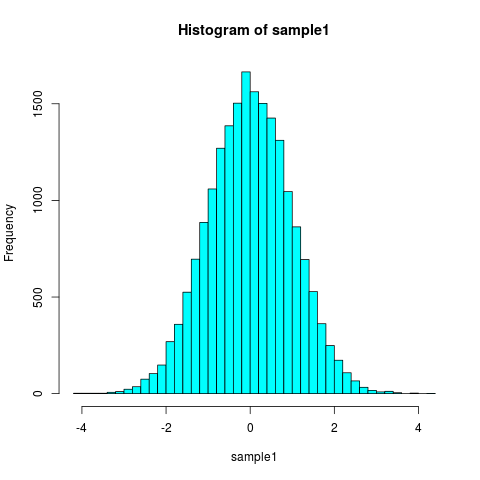
\includegraphics[width=\linewidth]{pic/que1_tenthousand_1.png}
 			 \caption{Using Box-Muller for 10000 sample} 
  			\label{fig:hist1}
		\end{figure}
		
		
			\begin{figure}
  			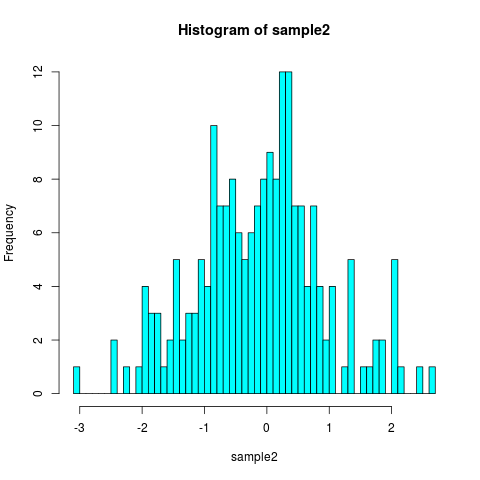
\includegraphics[width=\linewidth]{pic/que1_hund_2.png}
 			 \caption{Using Marsaglia-Bray for 100 sample} 
  			\label{fig:hist1}
		\end{figure}
	
			\begin{figure}
  			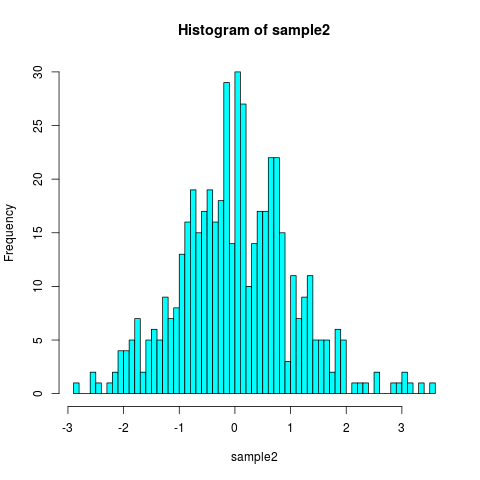
\includegraphics[width=\linewidth]{pic/que1_five-hund_2.png}
 			 \caption{Using Marsaglia-Bray for 500 sample} 
  			\label{fig:hist1}
		\end{figure}
	
			\begin{figure}
  			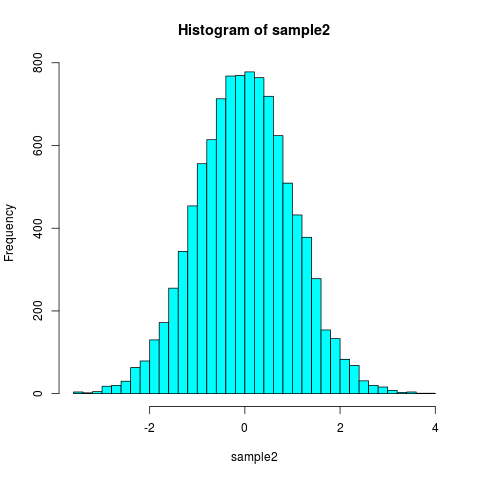
\includegraphics[width=\linewidth]{pic/que1_tenthousand_2.png}
 			 \caption{Using Marsaglia-Bray for 10000 sample} 
  			\label{fig:hist1}
		\end{figure}	
		
		\clearpage
		
		
		
	\section{Problem 2}
		In this problem we have to plot emirical and theoritical distribution of $N(0,5)$ and $N(5,5)$.
					
	\subsection{Source code generating Empirical and Theoritical Distributions}
		\lstinputlisting[language=R,firstline=1]{code/que2.R}
		
	\subsection{Generated Graphs}
	
			\begin{figure}[!ht]
  			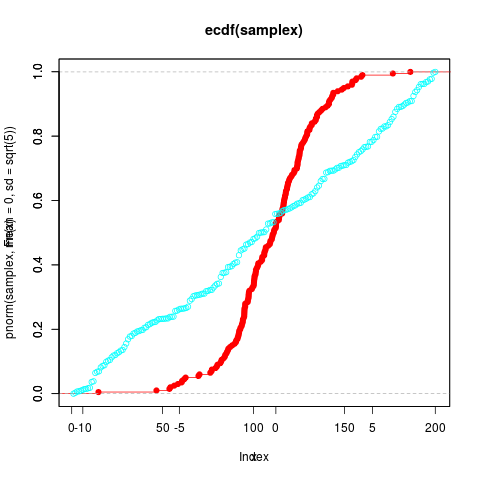
\includegraphics[width=\linewidth]{pic/que2_one.png}
 			 \caption{Plot of Emirical and Theoritical distribution of $N(0,5)$} 
  			\label{fig:hist1}
		\end{figure}
		
		\begin{figure}[!ht]
  			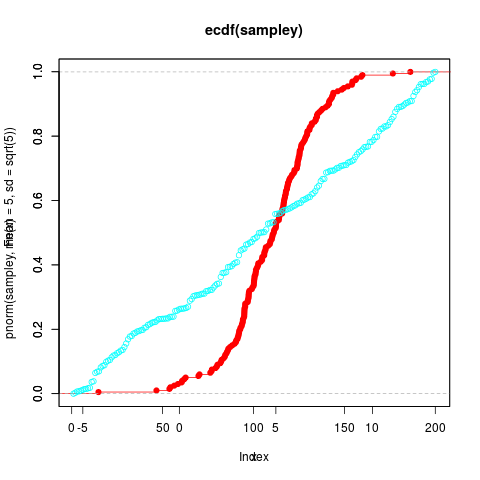
\includegraphics[width=\linewidth]{pic/que2_two.png}
 			 \caption{Plot of Emirical and Theoritical distribution of $N(5,5)$} 
  			\label{fig:hist1}
		\end{figure}
		
		\clearpage
		
		\section{Problem 3}
			In this problem we have to calculate the time taken to calculate Standard Normal distribution using Box-Muller and Marsaglia-Bray Mehods.
			
		\subsection{Source code for Box-Muller}
		\lstinputlisting[language=R,firstline=1]{code/que3-muller.R}	
	
		\subsection{Source code for Marsaglia-Bray}
		\lstinputlisting[language=R,firstline=1]{code/que3-bray.R}


		\subsection{Analysis}
			\paragraph{}
			Time taken for Box-Muller:  $0.0003612041 $
			
			\paragraph{}			
			Time taken for Masaglia-Bray:  $0.002064705$
		
			\paragraph{}
				We can cleary see that Box-Muller takes more time than Marsaglia Bray		
		\section{Problem 4}
			In this section we calculate number of rejections proportional to total sampled uniform random variables.
			
			\subsection{Source code for Solution}
		\lstinputlisting[language=R,firstline=1]{code/que4.R}		
		
		\subsection{Analysis}
			Here, rejection probability comes as 0.2092361 which is quite close to $1- \frac{pi}{4} =0.2146$
			
		
		

		\end{document}
		
		
		
			